\documentclass{beamer}

\mode<presentation>
{
  \usetheme{default}
  \usecolortheme{beaver}
  \setbeamercovered{transparent}
  \setbeamertemplate{caption}[numbered]
}

\usepackage{booktabs}
\usepackage{float}
\usepackage{siunitx}
\usepackage{subfloat}
\usepackage{subfig}
% \usepackage[labelsep=none,labelformat=empty]{caption}
\usepackage{caption}
% \usepackage{neuralnetwork}
\usepackage{tikz}

%\tikzstyle{process} = [rectangle, draw,
%    text width=3em, text centered, rounded corners = 3pt, minimum height=2em]

% \renewcommand{\tablename}{}
\newcommand{\ra}[1]{\renewcommand{\arraystretch}{#1}}

\title
{
    Gait Event Detection Using an LSTM Network
}

\subtitle
{
    10-701
    % Introduction to Machine Learning
    Project Presentation
}

\author
{
    Pablo Iturralde\\
    Yin Zhong\\
    Jakob Bauer
    % Pablo A. Iturralde,
    % Yin Zhong,
    % Jakob Bauer
}

\date
{
    April 22, 2015
}

% ==============================================================================

\begin{document}

\begin{frame}
  \titlepage
\end{frame}

\begin{frame}{Introduction}
    \begin{figure}[H]
        \begin{center}
        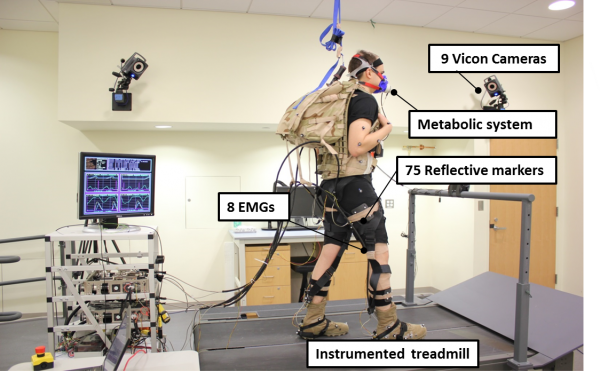
\includegraphics[height=.6\textheight]{figures/treadmill.png} \\
        \tiny from \url{http://biodesign.seas.harvard.edu/soft-exosuits}
        
        \small \textbf{Goal:}  Accurately detect gait events (heel strike, toe off) in video-based motion capture data of human walking gait
        \end{center}
    \end{figure}
\end{frame}

\begin{frame}{Introduction}
    \begin{itemize}
        \item \textbf{Problem:} Sequence labeling
        \begin{itemize}
            \item Input: 3D locus of 18 motion capture markers (54*N reals)
            \item Output: \{Left, Right\} $\times$ \{Heel Strike, Toe Off\} (4*N bools)
        \end{itemize}
        \item \textbf{Dataset:}
        \begin{itemize}
            \item 8 subjects $\times$ 3 trials $\times$ \num{10000} samples @ \SI{100}{\Hz}
            \item Ground truth from force plates on treadmills
        \end{itemize}
    \end{itemize}
\end{frame}

\begin{frame}{Our Approach}
    \begin{itemize}
        \item Objectives:
        \begin{itemize}
            \item Empirical feature-engineering should be minimal
            \item Number of manually-picked parameters (window size, threshold, filter cutoff, etc.) should be minimal
            \item Dependence of one gait cycle on those preceding it should be exploited
        \end{itemize}
        \item Proposed solution: LSTM-based RNN
        \begin{itemize}
            \item Recognition of periodic patterns even in presence of input noise
            \item Robust and precise learning of rhythmic timing
        \end{itemize}
    \end{itemize}
\end{frame}

\begin{frame}{Network architecture}
    \begin{figure}[H]
        \begin{center}
        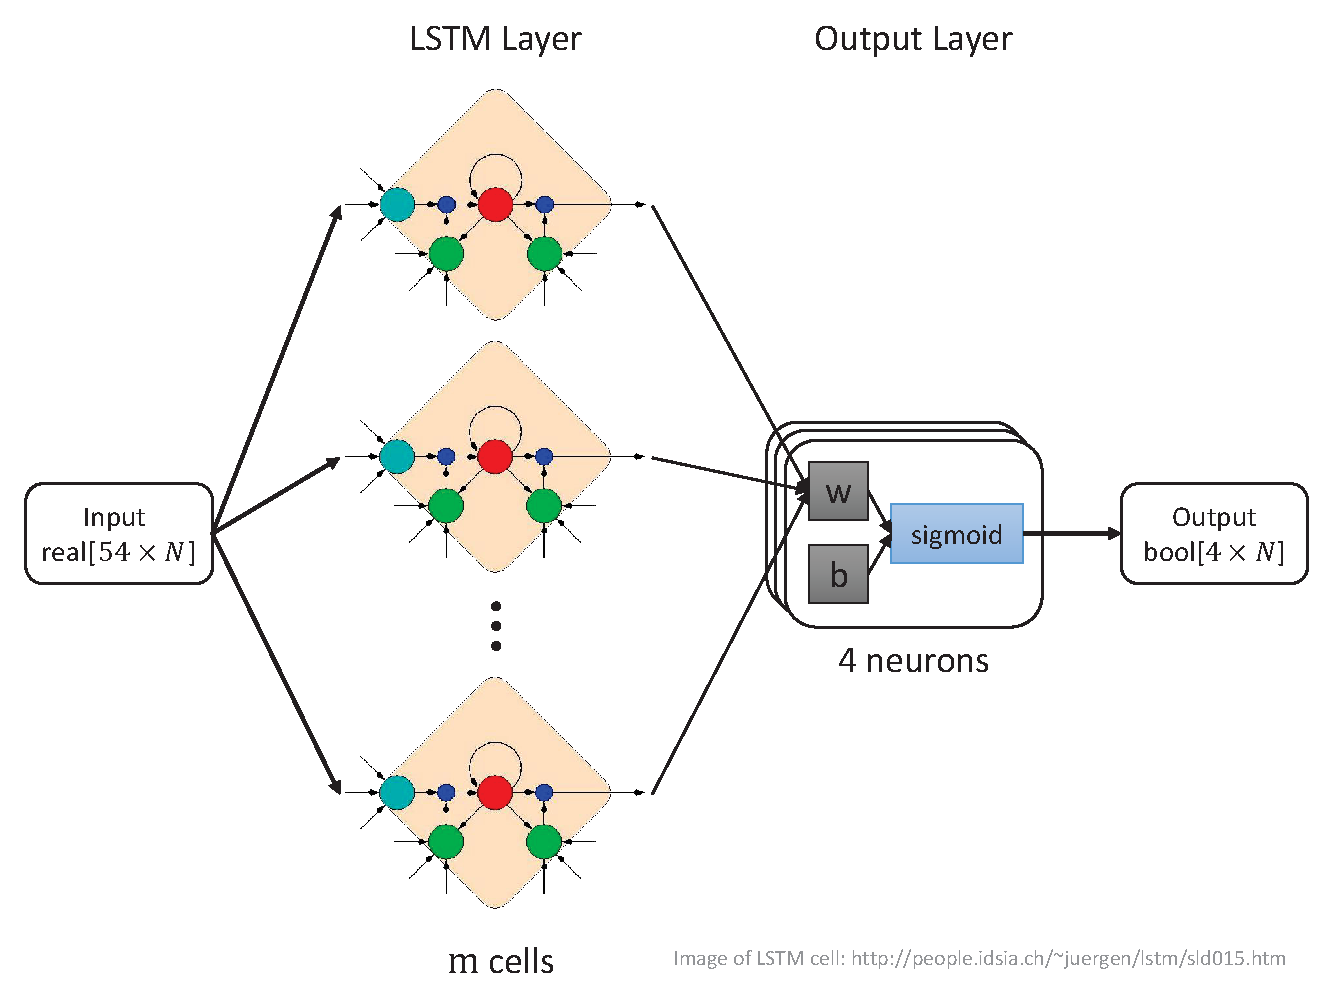
\includegraphics[height=.77\textheight]{figures/network.eps} \\
        \end{center}
    \end{figure}
\end{frame}

\begin{frame}{Implementation}
    \begin{itemize}
        \item Torch/Lua on AWS EC2 GPU instance (g2.2xlarge)
        \item Start with LSTM code example by de Freitas
        \begin{itemize}
            \item Adapt to our problem setup
            \item Problem: Does not converge out of the box
            \item Tweaks: Learning rate, mini-batch, regularization, etc.
        \end{itemize}
        \item Further work:
        \begin{itemize}
            \item Train on GPU (currently only runs on CPU cores)
            \item Explore other network architectures
            \item Improve time invariance
        \end{itemize}
    \end{itemize}
\end{frame}

\begin{frame}{Results}
    \begin{table}[H]
        \begin{center}
        \ra{1.2}
        % \footnotesize
        % \caption{Overview}
        \begin{tabular}{@{} lrrr @{}}
        \toprule
        % \multicolumn{4}{c}{\textbf{Random source}, $n=247$} \\
        {} & mean & std & mistake \\
        \midrule
        O'Connor  &     XXXXXXX &    XXXXXXX &    XXXXXXX \\
        Miller    &     XXXXXXX &    XXXXXXX &    XXXXXXX \\
        LSTM      &     XXXXXXX &    XXXXXXX &    XXXXXXX \\
        \bottomrule
        \end{tabular}
        \end{center}
    \end{table}
\end{frame}

\begin{frame}{Results}
    \begin{figure}
    \begin{center}
        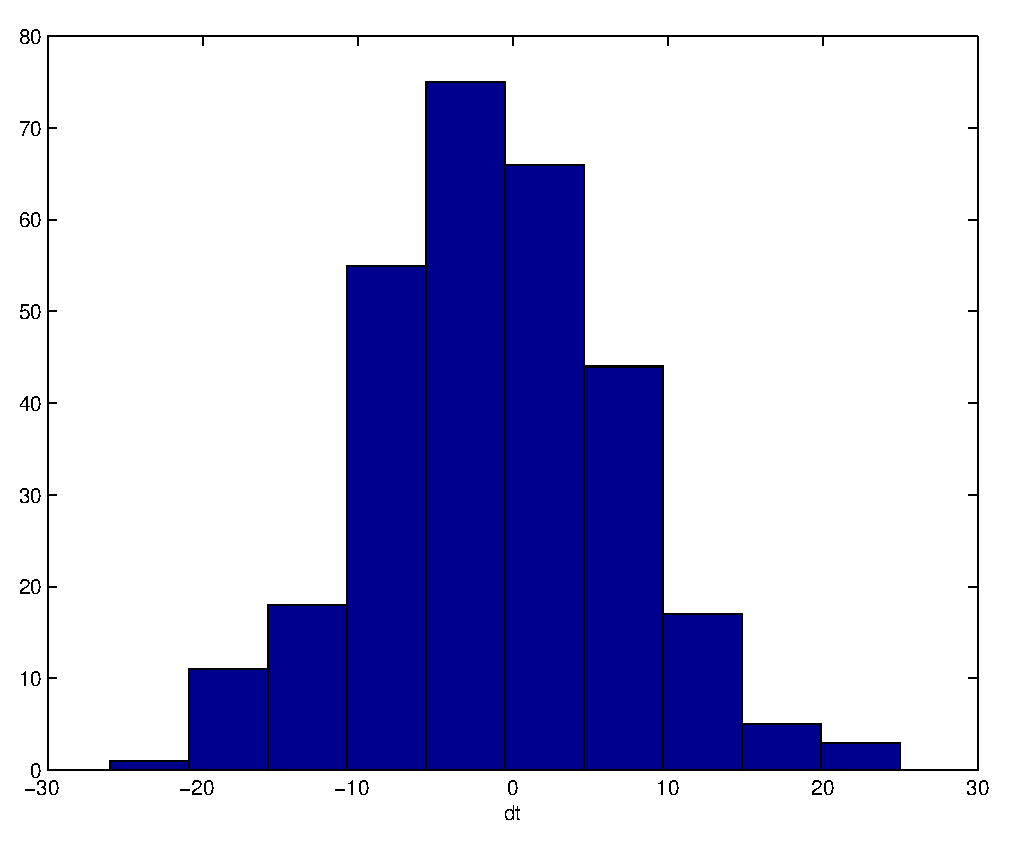
\includegraphics[width=0.75\textwidth]{figures/hist_miller.eps}
        \caption{Histogram Miller}
        \label{fig:hist_miller}
    \end{center}
    \end{figure}
\end{frame}

\begin{frame}{Q\&A}
    \Large
    \centering
    Thank you for your attention!
\end{frame}

\begin{frame}{Human Gait Cycle}
    \begin{figure}[H]
    \begin{center}
        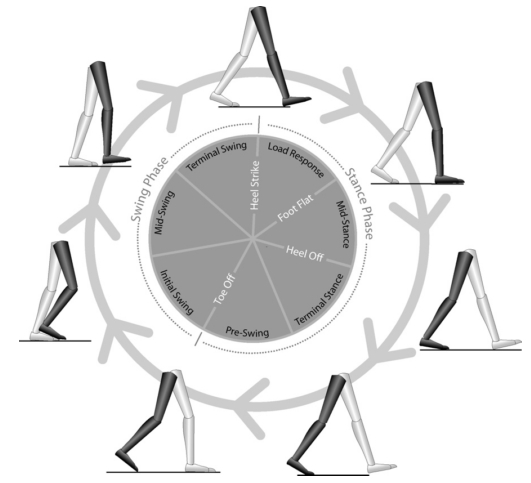
\includegraphics[height=.8\textheight]{figures/gait_events.jpg}
        \caption{Gait events [Rueterbories et al., 2010]}
        \label{fig:gait_events}
    \end{center}
    \end{figure}
\end{frame}


\end{document}
